\section{Suy luận kiểu - Type inference}
Sau khi đã hiện thực giải pháp Kiểm tra kiểu, nhận thấy rằng giải pháp này còn nhiều hạn chế và có thể cải tiến thêm, luận văn đã phát triển thêm một giải pháp mới tốt hơn, không bắt buộc người dùng phải thay đổi code của mình theo mẫu khai báo, đó là Suy luận kiểu. Với giải pháp này, bằng các phép phân tích dữ liệu, trình dịch ngược sẽ tự động tìm ra được các bộ biến được sử dụng trong chương trình. Ngoài bước chung của hai giải pháp là chỉnh sử trình dịch ngược để giữ nguyên tên biến đã được trình bày ở giải pháp trước, các bước của giải pháp Suy luận kiểu gồm có:
\begin{enumerate}
	\item Dùng một phương pháp phân tích luồng dữ liệu để biết được giá trị của thanh ghi ACC tại mỗi điểm của chương trình.
	\item Đi qua các câu lệnh sử dụng biến bit, ghi nhận giá trị hiện tại của thanh ghi ACc tại câu lệnh đó và đưa biến bit đó vào bộ biến phù hợp.
	\item Thêm vào các union tương ứng với bộ biến tìm ra được, thay thế các thanh ghi đại diện cho biến bit bằng truy xuất đến union tương ứng, cũng như thay thế vị trí sử dụng thanh ghi ACC.
\end{enumerate}
Như vậy, giải pháp này đã bỏ qua được bước đầu tiên, quy định mẫu khai báo, của giải pháp Suy luận kiểu. Ngoài ra, kỹ thuật phân tích Reaching definitions như đã trình bày ở chương trước có một số khuyết điểm, vì vậy, ở giải pháp này, chúng ta sẽ phân tích và tìm ra một kỹ thuật khác toàn diện hơn. Điều này sẽ được trình bày ở phần đầu tiên của chương, phần tiếp theo sẽ nói về cách quét các câu lệnh sử dụng biến bit và đưa thông tin vào một cấu trúc dữ liệu phù hợp.

\subsection{Phân tích Constant propagation}
Ở chương trước, phương phán phân tích Reaching definitions đã được đề cập đến, tuy nhiên, phương pháp này chỉ áp dụng được cho trường hợp gán một biến byte trực tiếp cho thanh ghi ACC, vì vậy ta cần tìm một phương pháp khác phù hợp hơn. Phương pháp này cần phải tính toán được chính xác giá trị hiện có của thanh ghi ACC cho dù biểu thức bên phải của phép gán là gì. Ngoài ra, nếu thanh ghi ACC có thể có mang những giá trị khác nhau ở một câu lệnh sử dụng bit, thì mặc nhiên nguyên tắc bị vi phạm. Như vậy, ta chỉ xét tới các trường hợp giá trị ở thanh ghi ACC là một giá trị cố định, có thể tính toán được trước khi thực thi chương trình. Từ các yêu cầu trên, ta kết luận được phương pháp phân tích phù hợp nhất trong trường hợp này là Lan truyền hằng số - Constant propagation. Phương pháp này cho phép tính toán giá trị của các biến, cho biết được gía trị đó có phải là một hằng số tại một thời điểm của chương trình hay không. Ví dụ như đoạn mã ban đầu \ref{list:listconstexam1}, có thể rõ ràng thấy giá trị của biến x là 14, nhưng ta không biết được giá trị thực sự của biến y, cũng như biểu thức trả về là bao nhiêu. Nhờ vào việc lan truyền hằng số, các giá trị này sẽ được tính toán, như trong đoạn mã \ref{list:listconstexam2} và \ref{list:listconstexam3}.
\begin{lstlisting}[caption={Đoạn mã trước khi thực hiện lan truyền hằng số},label={list:listconstexam1}, language=c++]
 int x = 14;
int y = 7 - x / 2;
return y * (28 / x + 2);
\end{lstlisting}
\begin{lstlisting}[caption={Đoạn mã sau khi thực hiện lan truyền hằng số cho biến y},label={list:listconstexam2}, language=c++]
int x = 14;
int y = 0;
return y * (28 / x + 2);
\end{lstlisting}
\begin{lstlisting}[caption={Đoạn mã sau khi thực hiện lan truyền hằng số cho biểu thức trả về},label={list:listconstexam3}, language=c++]
int x = 14;
int y = 0;
return 0;
\end{lstlisting}
Với phương pháp này, một biến có thể có ba giá trị sau:
\begin{itemize}
	\item Top: Nghĩa là chưa biết được biến có giá trị gì.
	\item Hằng số: Nghĩa là đã xác định được giá trị của biến là một hằng số.
	\item Bottom: Nghĩa là biến có thể mang những giá trị khác nhau, tuỳ thuộc vào luồng chạy của chương trình.
\end{itemize}

Ở bước khai báo ban đầu của giải thuật, tất cả các biến đều được truyền vào giá trị top (chưa biết), sau đó, trải qua quá trình phân tích thì giá trị của một biến có thể được xác định là hằng số (như giá trị của biến a tại câu lệnh số 3, đoạn mã \ref{list:listconstexam4}) hoặc là bottom (như giá trị biến a tại câu lệnh số 9, đoạn mã \ref{list:listconstexam5}).
\begin{lstlisting}[caption={Đoạn mã ví dụ biến có giá trị là hằng số},label={list:listconstexam4}, language=c++]
int a;
a = 4;
b = a*4;
\end{lstlisting}
\begin{lstlisting}[caption={Đoạn mã ví dụ biến có giá trị là bottom},label={list:listconstexam5}, language=c++]
int a;
int b;
cout<<"Enter b: ";
cin >> b;
if (b>15)
	a = 4;
else
	a = 5;
return a;
\end{lstlisting}

Như vậy, khi áp dụng vào trình dịch ngược Boomerang, mục tiêu của giải thuật này là để tìm ra được ở mỗi điểm của chương trình, giá trị thật sự của địa chỉ vùng nhớ mà thanh ghi ACC đang mang là gì.

Có nhiều cách thực hiện Constant propagation, vì trong Boomerang, có một giai đoạn code trung gian được giữ ở dạng SSA, nên ta sẽ chọn cách phân tích Sparse constant propagation để giảm thiểu thời gian xử lý. Và việc phân tích Constant propagation này sẽ được thực hiện ở cuối giai đoạn SSA, khi các phân tích khác đã hoàn tất. Giải thuật của phân tích Sparse constant propagation gồm có các bước được trình bày ở hình \ref{fig:constantpropagationalgo}

\begin{figure}
	\centering
	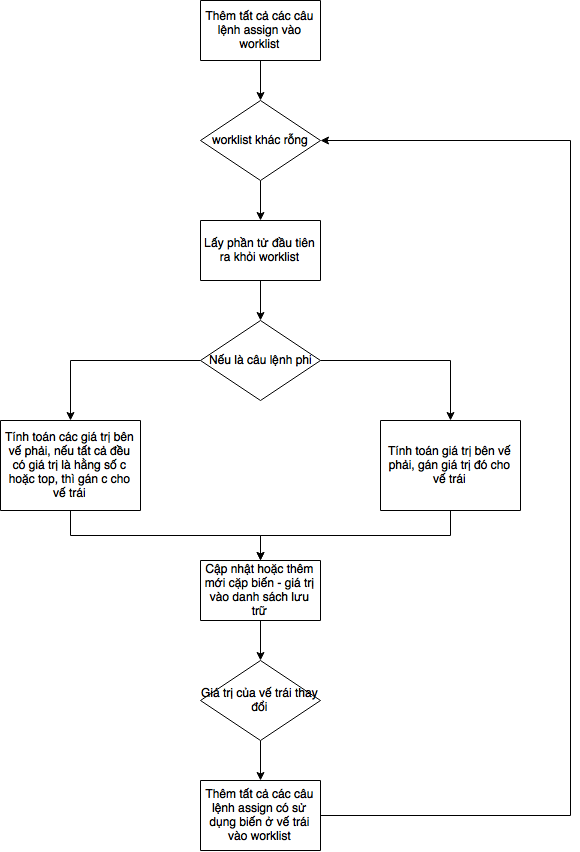
\includegraphics[scale=0.75]{image/constantPropagationAlgo}
	\caption{Giải thuật Constant propagation đã được điều chỉnh phù hợp với yêu cầu của trình dịch ngược}
	\label{fig:constantpropagationalgo}
\end{figure}

Để thể hiện giá trị của một biến có thể thuộc ba loại là top, hằng số hoặc bottom, ta sẽ tạo ra một class mới trong Boomerang, đó là ConstantVariable. Đoạn mã của class này được trình bày bên dưới.
\begin{lstlisting}[caption={Đoạn mã thể hiện class ConstantVariable},label={list:listconstexam5}, language=c++]
class ConstantVariable{
	public:
	int type; //1: top, 2: constant, 3: bottom
	Exp* variable;
	ConstantVariable(){
		type = 3;
	}
};
\end{lstlisting}
Như vậy, ta có thể thấy kết quả của giải thuật này là tạo ra được một sơ đồ map giữa một biến SSA và một thực thể ConstantVariable thể hiện giá trị của biến đó. \\

Ngoài ra, ta sẽ áp dụng code pattern Visitor để tính toán được giá trị của các biểu thức nằm ở vế phải của lệnh gán. Visitor đó được đặt tên là EvalExpressionVisitor. Vì các biểu thức có thể viết ở mức assembly khá đơn giản, nên ta chỉ cần viết hàm visit cho các loại biểu thức sau:

\begin{itemize}
	\item Const: Là biểu thức hằng số. Hàm visit này chỉ đơn giản trả về giá trị hằng số nếu đây là một hằng số nguyên.
	\item Binary: Là biểu thức có 2 vế. Hàm visit sẽ visit từng vế của biểu thức, và nếu cả hai vế đều là hằng số, thì sẽ thực hiện phép tính cộng trừ nhân chia hai hằng số đó để ra được kết quả cuối cùng.
	\item RefExp: Loại biểu thức này chứa một biểu thức khác, kèm theo câu lệnh khai báo biểu thức đó. Cụ thể, ta chỉ xét loại RefExp có biểu thức con là một biến. Ta sẽ tìm trong sơ đồ hiện tại để lấy ra giá trị của biến đó. Nếu không có trong sơ đồ, ta sẽ tìm trong bảng lưu trữ dữ liệu các câu lệnh \#DEFINE để xem đó có phải là một biến đã được khai báo trước trong chương trình đầu vào không.
	\item TypedExp: Loại biểu thức để ép kiểu một biểu thức nào đó thành kiểu mong muốn. Với trường hợp này, ta sẽ visit biểu thức con và trả về giá trị của biểu thức đó.
\end{itemize}


Như vậy, với phương pháp phân tích này, ta có thể giải quyết được vấn đề vế phải của phép gán thanh ghi ACC không chỉ đơn giản là một biến byte. Ngoài ra, nó còn nhận biết được các biểu thức có giá trị giống nhau mặc dù hình thức bên ngoài khác nhau. Xem ví dụ các câu lệnh ở đoạn mã \ref{list:listdiffassignacc}. Câu lệnh gán số 1 và số 2 thực chất đều gán cho ACC giá trị vùng nhớ có địa chỉ quy định bởi biến OPTIONS. Nếu thực hiện phân tích Reaching definitions ở giải pháp trước, trình dịch ngược sẽ không thể biết được điều này. Tuy nhiên, ở giai đoạn này, vì trình dịch ngược sẽ tính toán được ở cả hai câu lệnh, ACC đều mang giá trị của vùng nhớ có địa chỉ là 38H. Và ở những bước tiếp theo, trình dịch ngược sẽ đối chiếu giá trị 38H với bảng lưu trữ dữ liệu và biết được biến OPTIONS đại diện cho giá trị đó.

\begin{lstlisting}[caption={Một số câu lệnh gán cho ACC có giá trị vế phải bằng nhau},label={list:listdiffassignacc}]
\#DEFINE OPTIONS \#38H
...
MOV ACC, OPTIONS
MOV ACC, 38H
\end{lstlisting}

Một lưu ý là trong trường hợp này, ta không xét đến giá trị của thanh ghi ACC, mà ta chỉ xét đến giá trị của địa chỉ vùng nhớ thanh ghi ACC đang lưu giữ. Như vậy, chỉ có các câu lệnh dạng MOV ACC, [biểu thức] sẽ được xét đến. Khi gặp câu lệnh gán có dạng MOV ACC, \#[biểu thức] thì đoạn mã phân tích sẽ xem như giá trị của ACC không phải là hằng số (bottom).
\subsection{Quét các câu lệnh sử dụng biến bit}

Sau khi đã biết được giá trị địa chỉ vùng nhớ mà thanh ghi ACC đang nắm giữ, ta sẽ chuyển sang bước quét các câu lệnh sử dụng biến bit. Ở bước này, ta vẫn sẽ sử dụng lại cấu trúc dữ liệu UnionDefine đã giới thiệu ở chương trước. Tuy nhiên, sau quá trình phân tích, ta chỉ biết được giá trị, chứ không biết được biến byte nào đang lưu trữ giá trị đó. Và để tăng tốc độ chương trình, ta sẽ lưu giá trị đó vào UnionDefine chứ không lưu biến byte, chỉ khi kết thúc quá trình quét dữ liệu, ta mới truy cập vào bảng lưu trữ các câu lệnh \#DEFINE, so sánh và tìm ra được biến byte nào tương ứng với các giá trị đó. Như vậy, cần có thêm một trường để lưu giá trị trực tiếp trong UnionDefine.

%đoạn mã mới của unionDefine

Quá trình quét câu lệnh và thu thập dữ liệu của giải pháp Suy luận kiểu cũng tương tự như giải pháp Kiểm tra kiểu, nhưng thay vì ghi nhận biến bit và biến byte rồi kiểm tra chúng có cùng một bộ như khai báo hay không, ta sẽ kiểm tra trước hai biến đó có vi phạm nguyên tắc sử dụng hay không (ví dụ như biến bit đó đã thuộc một bộ khác trước đó, hoặc ở bit vị trí đó của bộ biến của biến byte đã ghi nhận một biến bite khác), nếu không thì ta sẽ ghi nhận mối quan hệ này vào danh sách UnionDefine đang lưu trữ.

%sơ đồ các bước quét dữ liệu

Sau khi đã quét hết các câu lệnh ở các procedure, trước khi chuyển đổi các UnionDefine thành các khai báo ở ngôn ngữ C và thêm vào danh sách các biến toàn cục của program như giải pháp trước, ta phải thêm vào một bước chuyển đổi từ giá trị thành biến byte đại diện cho giá trị đó. Điều này có thể được thực hiện bằng cách chạy vòng lặp qua bảng lưu trữ các câu lệnh \#DEFINE đã được thiết lập từ quá trình parse mã đầu vào.

%ví dụ tìm biến byte ứng với giá trị

Nếu như có một giá trị nào đó chưa được khai báo ở câu lệnh \#DEFINE, ta sẽ đặt tên mới cho biến byte đó là LOCATION\_[giá trị].

%ví dụ đặt tên mới cho biến byte

Bước cuối cùng cũng tương tự giải pháp trước, đó là thay thế. Ngoài việc bỏ các câu lệnh gán thanh ghi ACC, thay thế biến ACC bằng các biến byte tương ứng, ta còn có thêm một bước là thay thế các biến bit bằng các truy xuất tới union. Ở giải pháp trước, vì ta đã biết ngay từ đầu biến bit nào thuộc chung bộ với biến byte nào, nên ở giai đoạn giải mã, khi gặp một biến bit ta đã thay thế nó bằng truy xuất tới union. Còn ở giải pháp này, ta không biết được các bộ biến, nên ở giai đoạn giải mã ta sẽ xem các biến bit như một biến độc lập. Sau khi đã tìm ra được các bộ biến, ta mới thực hiện thay thế chúng.

%ví dụ thay thế biến bit

Ngoài thay thế các biến bit, đoạn mã này còn quét các vị trí người dùng gọi trực tiếp một bit của thanh ghi ACC, ví dụ như ACC.1. Với trường hợp này, đoạn mã sẽ tìm biến bit ở vị trí số một của biến byte tương ứng với giá trị thanh ghi ACC, và thay thế đoạn mã truy xuất trực tiếp đó bằng tên biến bit. 

%ví dụ đoạn mã sử dụng truy xuất trực tiếp biến bit

Như vậy, giải pháp này đã giải quyết phần lớn các vấn đề đặt ra của bài toán. 

%một đoạn mã đầu vào và đoạn mã đầu ra của trình dịch ngược